\documentclass[]{interact}
\usepackage{epstopdf}
\usepackage{subfigure}
\usepackage{natbib}
\bibpunct[, ]{(}{)}{,}{a}{}{,}
\renewcommand\bibfont{\fontsize{10}{12}\selectfont}
\theoremstyle{plain}
\newtheorem{theorem}{Theorem}[section]
\newtheorem{lemma}[theorem]{Lemma}
\newtheorem{corollary}[theorem]{Corollary}
\newtheorem{proposition}[theorem]{Proposition}
\theoremstyle{definition}
\newtheorem{definition}[theorem]{Definition}
\newtheorem{example}[theorem]{Example}
\theoremstyle{remark}
\newtheorem{remark}{Remark}
\newtheorem{notation}{Notation}
\usepackage{color,soul}

\begin{document}

	\title{Estimating real-time highstreet footfall from Wi-Fi probe requests}
	\author{
		\name{ Balamurugan Soundararaj\textsuperscript{a}\thanks{CONTACT Balamurugan Soundararaj. Email: s.bala@ucl.ac.uk}, James Cheshire\textsuperscript{a} and Paul Longley\textsuperscript{a} }
		\affil{\textsuperscript{a}Department of Geography, University College London, United Kingdom.}
	}
	\maketitle
	\begin{abstract}
		% ==============================================================================
% DOCUMENT HEADER
% ==============================================================================

\documentclass[11t, a4paper, twocolumn]{article} 
\usepackage[english]{babel}
\usepackage{microtype}
\usepackage{amsmath,amsfonts,amsthm}
\usepackage[svgnames]{xcolor}
\usepackage[hang, small, labelfont=bf, up, textfont=it]{caption}
\usepackage{booktabs}
\usepackage{lastpage}
\usepackage{graphicx}
\usepackage{enumitem}
\setlist{noitemsep}
\usepackage{sectsty}
\allsectionsfont{\usefont{OT1}{phv}{b}{n}}
\usepackage{lipsum}
\usepackage{geometry}
\geometry{
	top=1cm,
	bottom=1.5cm,
	left=2cm,
	right=2cm,
	includehead,
	includefoot
}
\setlength{\columnsep}{7mm}
\usepackage[T1]{fontenc}
\usepackage[utf8]{inputenc}
\usepackage{XCharter}
\usepackage{fancyhdr}
\pagestyle{fancy}
\renewcommand{\headrulewidth}{0.0pt}
\renewcommand{\footrulewidth}{0.25pt}
\renewcommand{\sectionmark}[1]{\markboth{#1}{}}
\lhead{}
\chead{\textit{\thetitle}}
\rhead{}
\lfoot{}
\cfoot{}
\rfoot{\footnotesize Page \thepage\ of \pageref{LastPage}}
\fancypagestyle{firstpage}{
	\fancyhf{}
	\renewcommand{\footrulewidth}{0pt}
}
\newcommand{\authorstyle}[1]{{\large\usefont{OT1}{phv}{b}{n}\color{Black}#1}}
\newcommand{\institution}[1]{{\footnotesize\usefont{OT1}{phv}{}{sl}\color{Black}#1}}
\usepackage{titling}
\newcommand{\HorRule}{\color{Black}\rule{\linewidth}{0.75pt}}
\pretitle{
	\vspace{-30pt}
	\HorRule\vspace{10pt}
	\fontsize{30}{34}\usefont{OT1}{phv}{b}{n}\selectfont
	\raggedright
	\color{Black}
}
\posttitle{\par\vskip 15pt}
\preauthor{}
\postauthor{
	\vspace{10pt}
	\par\HorRule
	\vspace{5pt}
}
\usepackage{lettrine}
\usepackage{fix-cm}
\newcommand{\initial}[1]{
	\lettrine[lines=3,findent=4pt,nindent=0pt]{
		\color{DarkGoldenrod}
		{#1}
	}{}
}
\usepackage{xstring}
\newcommand{\lettrineabstract}[1]{
	\StrLeft{#1}{1}[\firstletter]
	\initial{\firstletter}\textbf{\StrGobbleLeft{#1}{1}}
}
\usepackage[backend=bibtex,style=numeric,natbib=true]{biblatex}
\addbibresource{ref.bib}
\usepackage[autostyle=true]{csquotes}


\title{Estimating real-time high treat  footfall from Wi-Fi probe requests}
\author{
	\authorstyle{
		Balamurugan Soundararaj\textsuperscript{1}, 
		James Cheshire\textsuperscript{1} and 
		Paul Longley\textsuperscript{1}}
	\newline\newline
	\textsuperscript{1}\institution{
		Department of Geography, 
		University College London, 
		United Kingdom}
}
\date{\today}

% ==============================================================================
% DOCUMENT BODY
% ==============================================================================

\begin{document}

	\maketitle
	\thispagestyle{firstpage}

	In the past decade, Wi-Fi has emerged as the most commonly used technolo
gy in providing internet access to mobile devices such as smartphones, tablets a
nd laptops in public and private spaces. This has resulted in multiple Wi-Fi net
works being available at almost every location in urban environments. Traversing
 through this overlapping mesh of Wi-Fi networks, modern mobile devices with Wi-
Fi antennae regularly broadcast a special type of signal known as probe requests
, in order to discover available Wi-Fi networks and switch seamlessly between th
em. This is a hardware level signal which was standardised by IEEE 802.11b/g spe
cification, to relay information about the source mobile device to any Access Po
int (AP) available around it. Since this is the first step in establishing a con
nection between any two devices, it is a standard feature of any device which us
es a Wi-Fi radio to communicate. This makes these probe requests an open, passiv
e, continuous, and wireless source of data available at any urban location. More
over, the data can provide us with clues to understand the number of people pres
ent in the immediate surrounding in real-time and with high granularity \citep{f
reud2015,konto2017}. In this paper, using a set of probe requests collected at a
 high street location in London along with manually counted data, we demonstrate
 that pedestrian footfall can be estimated with considerable accuracy without in
fringing on the privacy of the mobile users involved.

	\begin{figure*}
		\begin{center}
			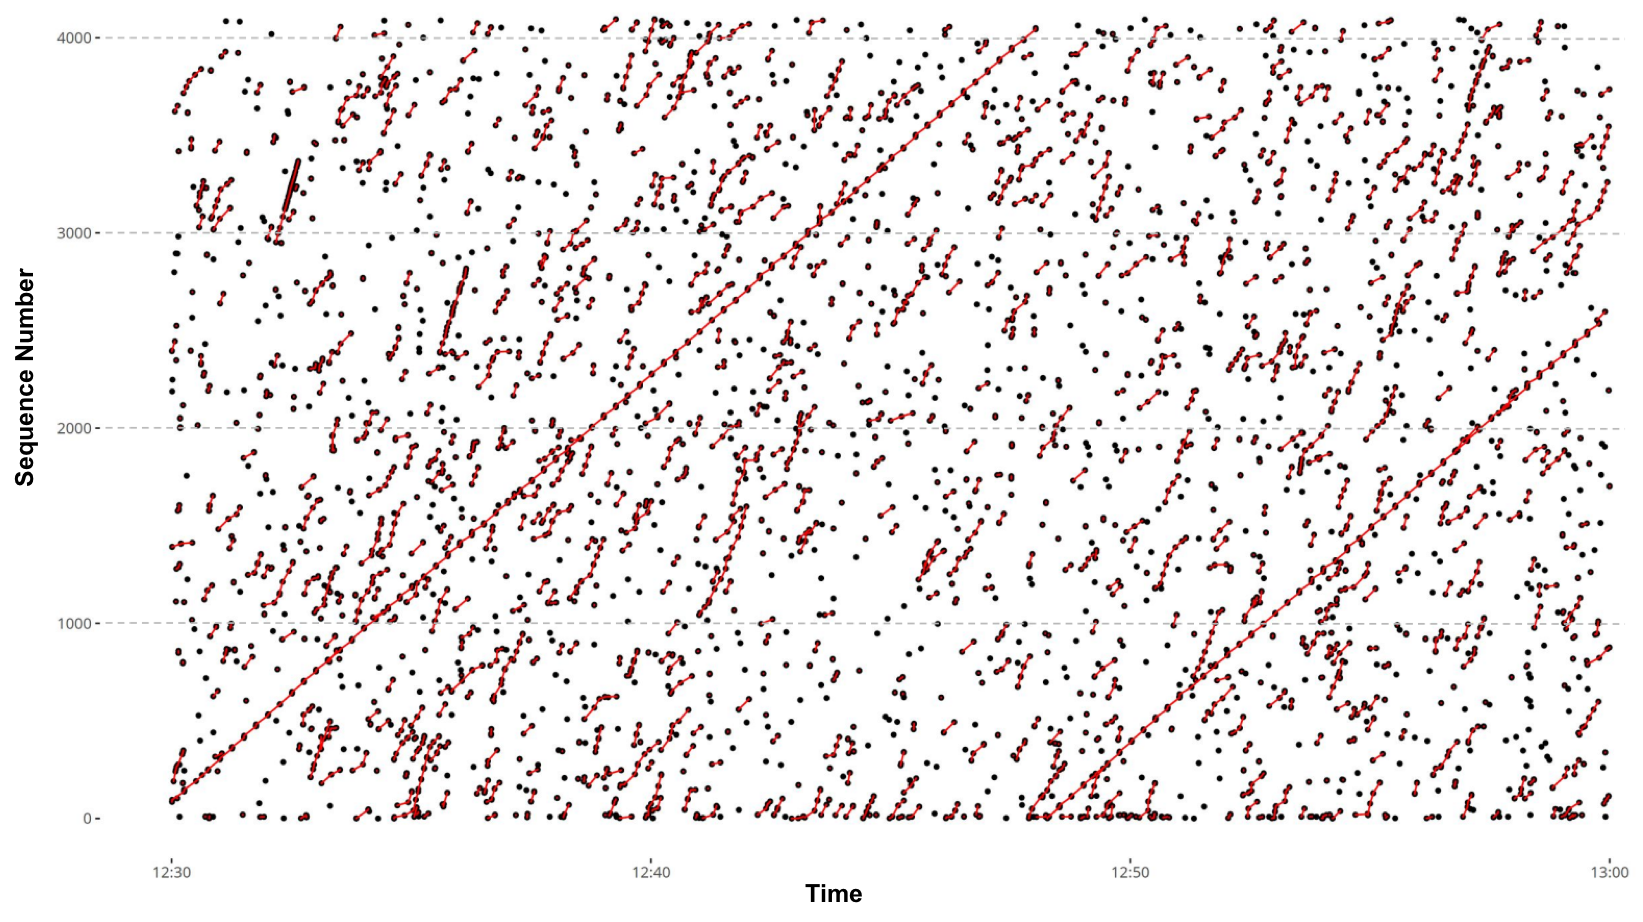
\includegraphics
				[width=0.8\textwidth,trim=4 4 4 4,clip]
				{outputs/clustering_2.png}
			\caption{Clustering probe requests based on increasing s
equence
			numbers present in them.}
			\label{fig}
		\end{center}
	\end{figure*}

	There have been numerous attempts at using Wi-Fi to measure the volume a
nd movement of people in the built environment for various applications \citep{z
arim2006,sap2015,reki2007}. Though most research obtains feasible and favorable 
results, in recent years, one of the major challenges faced in such attempts has
 been the MAC address randomisation process. This process aims to protect the us
ers’ privacy by anonymising the only globally identifiable portion of the prob
e requests, which results in a set of probe requests generated by the same devic
e with different random MAC addresses \citep{green2008}. There have been various
 successful attempts by researchers to breaking this randomisation process in or
der to extract real MAC addresses, \citep{martin2017} but this usually results i
n serious risk of infringement of the privacy of the users of the mobile devices
. There is a clear gap in the research for exploring methodologies which enable 
us to estimate the number of unique mobile devices from a set of anonymised prob
e requests, without the need to reveal their original MAC addresses.

	A pilot survey was conducted on Oxford Street in London in December 2017
, where two sets of data were collected on pedestrian footfall. These datasets w
ere collected through Wi-Fi sensing and manual counting in parallel. The Wi-Fi s
ensor collected all the probe requests which were broadcast around the area, and
 recorded the following data: the time-stamp at which they were collected, the M
AC address of the source mobile device (anonymised using a hashing algorithm), t
he organisationally unique identifier (OUI) of the manufacturer of the device, t
he total length of the signal in bits, the strength of the signal reported by th
e mobile device in dBm, the sequence number of the signal, the duration for whic
h the signal was transmitted, the service set identifier (SSID) of the access po
int targeted by the probe request, and the length of the extra information (tags
) embedded in the packets. The manual count was undertaken using an Android appl
ication on a mobile phone: the researcher touched the phone’s screen every tim
e an individual pedestrian footfall was counted, and this was recorded as a time
-stamp. 

	Being located at one of the busiest retail locations in the United Kingd
om, the WiFi sensor captured approximately 60,000 probe requests over a 30 minut
es interval, and 3,722 people were counted manually. When we aggregated the prob
e requests by their MAC address for every minute, the difference between the sen
sor counts and the manual counts was observed to be on average 425\%. This sugge
sted that there was a large amount of noise in the data which might have include
d signals from devices outside the area where themanual count was conducted, as 
well as anonymised probe requests from the same devices but with different MAC a
ddresses. An initial analysis revealed that the fields - SSID and tags - were ve
ry sparse and did not provide much information for our cleaning process. In addi
tion, the duration field was closely related to the length of the probe request 
and provides no new information. Therefore, we removed these fields from further
 analysis.

	We eliminated the noise from devices outside the area of interest by rem
oving all the probe requests which reported a "low" signal strength. This classi
fication of "high" vs "low" was performed using a k-means classification algorit
hm. The cut-off point for the collected data was -71 dBm. This process of filter
ing was highly effective and reduced the difference between the sensor counts an
d manual counts to 30\%. We observed that around 55\% of all probe requests coll
ected were anonymised. We assigned the hashed MAC address the unique identifier 
for the remaining 45\% and investigated the anonymised probe requests further.

	We then used the fields - OUI, lengths and sequence number - to tackle t
he noise from devices which anonymised the probe requests. OUI and length were u
sed to split the dataset into groups of probe requests from similar devices, and
 each subset was classified further using a graph based clustering algorithm whe
re each cluster corresponded to a unique device. The algorithm created a graph w
here the probe requests represented the nodes, and links are created between the
m based on the following rules: 
		
	\begin{enumerate}
		\item A link could go only forward in time. 
		\item A link could exist between nodes with a maximum time diffe
rence of $\alpha$ (time threshold).
		\item A link could go from low to high sequence numbers.
		\item A link could exist between nodes with a maximum sequence n
umber difference of $\beta$ (sequence threshold).
		\item A node could have only one incoming link and one outgoing 
link, which is the shortest of all such possible links.
	\end{enumerate}

	The nodes were then classified based on the unique connected component t
hey belonged to. This classification was assigned as the unique identifier for t
he anonymised probe requests. Figure \ref{fig} shows the clustering process: the
 black dots show the probe requests and the red lines connect them into clusters
 representing those which were generated by the same device. We finally combined
 both normal and anonymised probe requests, aggregated them based on their uniqu
e identifier, and removed repeating probe requests which reduced the difference 
between the sensor counts and the manual counts to -18\%.

	It is important to note that the filtering process was done based soley 
on the information present in the probe requests and their temporal distribution
. This ensured that although the mobile devices were uniquely identified, there 
was no further personal data generated by linking the probe requests to the user
s of the mobile devices. This method essentially gave us a way to estimate the f
ootfall in real-time without identifying or tracking the mobile devices themselv
es.

	This Wi-Fi based footfall counting methodology offers a large number of 
applications and benefits for real time spatial analysis. Since Wi-Fi based sens
ors are inexpensive and the data model is scalable, it is possible to use this m
ethodology for a large network of sensors to gather granular data on pedestrian 
footfall. Projects such as SmartStreetSensors \citep{sss2016}, may utilise this 
methodology to overcome the challenges introduced by the implementation of MAC a
ddress randomisation. Such precise and granular data also enables us to confiden
tly model the pedestrian flow in urban road networks, and will be an indispensab
le tool in the smart city framework. It can also be used to understand and class
ify geographical areas based on the spatio-temporal distribution of the volume o
f activity in them.

	\printbibliography[title={References}]

\end{document}
 \end{abstract}
	\begin{keywords}
		Highstreet footfall; Wi-Fi Probe requests; Sensors; MAC Randomisation \end{keywords}
	\section{Introduction}\label{introduction}
		In the past decade Wi-Fi has emerged as the most commonly used technology in providing high speed internet access to mobile devices such as smartphones, tablets and laptops in public and private spaces. This has resulted in multiple Wi-Fi networks being available at almost every location in dense urban environments. Traversing through this overlapping mesh of Wi-Fi networks, modern mobile devices with Wi-Fi antennae regularly broadcast a special type of signal known as 'Probe Requests', in order to discover Wi-Fi networks available to them. This helps these devices to connect and switch between the WiFi networks seamlessly.

Probe requests are low level signals standardised by IEEE 802.1b/g specification as the first step in establishing a Wi-Fi based connection between two devices and is implemented in any Wi-Fi capable device irrespective of the manufacturer or the model. This ubiquity and standardisation make them an excellent source of open, passive, continuous, and wireless data generated by Wi-Fi capable devices present at any given time and location. Considering the unprecendented levels of mobile device ownership in recent years, we can in turn use this data to understand the population distribution in highly dynamic urban environments with high spatial and temporal granularity \citep{freud2015,konto2017}.

While a Wi-Fi based method to collect data offers us various advantages such as, easy scalability and efficiency in terms of cost and time, It also introduces few systematic biases, uncertainities in the collected data along with the serious risk of infringing on the privacy of the mobile users. In this paper, using a set of probe requests and manual counts collected at various high street locations across London, we demonstrate that pedestrian footfall at these locations can be estimated with considerable precision and accuracy while protecting the privacy of the pedestrians.

	\section{Previous Work}\label{previous_work}
		In the past decade, Wi-Fi has emerged as one of the most commonly used
technologies in providing high speed internet access to mobile devices such as
smartphones, tablets and laptops in public and private spaces
\citep{torrens2008wi}. This has resulted in multiple Wi-Fi networks being
available at almost every location in dense urban environments. Traversing
through this overlapping mesh of Wi-Fi networks, modern mobile devices with
Wi-Fi network interfaces regularly broadcast a special type of signal known as
`Probe Requests' in order to discover the Wi-Fi networks available to them.
This helps these devices to connect and switch between the Wi-Fi networks
seamlessly.

Probe requests are low level signals standardised by IEEE 802.11 specification
\citep{ieee2016} for service discovery, and are implemented in any Wi-Fi
capable device irrespective of the manufacturer or the model. This ubiquity and
standardisation makes them an excellent source of open, passive, continuous,
and wireless data generated by Wi-Fi capable devices present at any given time
and location. Considering the unprecendented levels of mobile device ownership
in recent years, we can, in turn use this data to understand the population
distribution in highly dynamic urban environments with high spatial and
temporal granularity \citep{freud2015, konto2017}. While a Wi-Fi based method to
collect data offers us various advantages such as, easy scalability and
efficiency in terms of cost and time, it also introduces few systematic biases
and uncertainities in the collected data along with the serious risk of
infringing on the privacy of the mobile users. In this paper, using a set of
probe requests and manual counts collected at various high street locations
across London, we demonstrate that pedestrian footfall at these locations can
be estimated with considerable precision and accuracy while protecting the
privacy of the pedestrians.

Unlike GPS, the location of the Wi-Fi enabled mobile device cannot be directly
inferred from Wi-Fi, however there are reliable methods to triangulate the
location of mobile devices from the locations of known access points (AP) and
the signal strength reported by them \citep{he2003range, moore2004robust,
lamarca2005place}. This can overcome the usual shortcoming of GPS, which
struggles for precision and accuracy in indoor and densely built environments
\citep{zarim2006, kawaguchi2009wifi, xi2010locating}. Utilising this, we can
easily and quickly estimate trajectories of the mobile devices
\citep{musa2012tracking} which can be used similary to the
GPS trajectories to understand individual travel patterns \citep{reki2007,
Sap2015}, crowd behaviour \citep{abedi2013bluetooth, mowafi2013tracking},
vehicular \citep{lu2010vehicle} and pedestrian movement
\citep{xu2013pedestrian, fukuzaki2014pedestrian, wang2016gait}. Such data can
also be used in transportation planning and management to estimate travel time
\citep{musa2011wiflow} and real time traffic monitoring
\citep{abbott2013empirical}. Using techniques demonstrated by
\cite{franklin2006passive} and \cite{pang2007802}, along with information
present in the probe requests, one can even model interactions between the
users \citep{cheng2012inferring, barbera2013signals, cunche2014know,
cunche2014linking} such as predicting which of them are most likely to meet
again \citep{cunche2012know}. Using the semantic information present in these
probe requests it even is possible to understand the nature of population at a
large scale \citep{di2016mind}. 

Although extensive research has been carried out on this subject with feasible
and favorable results, in recent years, one of the major challenges faced in
such attempts has been the increasing attempt by mobile phone manufacturers to
protect their users’ privacy by anonymising the globally identifiable portion
of the probe requests \citep{green2008}. Various methods have been devised to
overcome this anonymisation process such as estimating the device model
information from a known dataset of manufacturers and device behaviours
\citep{martin2016decomposition}; Scrambler attack using a small part of the
physical layer specification for Wi-Fi \citep{vo2016, bloessl2015scrambler};
and timing attack where the packet sequence information along with information
elements present in the probe request frame is used \citep{matte2016,
cheng2016can}. A combination of these methodologies has been proven to produce
de-anonymised globally unique device information \citep{vanhoef2016,
martin2017}. These approaches usually result in serious risk of breach of
privacy of the users of the mobile devices by revealing their
identifiable personal information.

There is a clear gap in the research for exploring methodologies for estimating
the number of unique mobile devices from a set of anonymised probe requests,
without the need to reveal their original device information. Such a technique
has various applications such as uncovering the urban wireless landscape
\citep{rose2010mapping}, revealing human activity at large scales
\citep{qin2013discovering}, estimating pedestrian numbers in crowds
\citep{schauer2014estimating, fukuzaki2015statistical}, and even counting
people in hyper local scales such as queues \citep{wang2013measuring}. With
enough infrastructure to collect such information we can even aim to generate a
real-time census of the city \citep{konto2017}. With this background, we set
out to devise and implement a methodology to reliably estimate human activity
such as pedestrian footfall from Wi-Fi probe requests without risking a breach
of privacy of the users involved.

	\section{Methodology}\label{methodology}
		The primary aim of this research is to enable us to collect a series of probe requests and process them into an usable pedestrian footfall count. We do this by using a Wi-Fi receiver to collect probe requests broadcasted by mobile devices, filtering out the background noise and aggregating them based on the device that generated them. We begin by looking at the characteristics of probe requests in detail, device a methodology to collect these probe requests in public areas, examine the systemic biases and uncertainties in the data collection method and device data processing methods to overcome these challanges. Finally we compare the processed footfall counts to the ground truth recorded by primary surveys.

Probe requests are a special type of management packets broadcast by Wi-Fi enabled devices as part of the various functions such as scanning for available access points (AP), quick geo-location by triangulation based known APs, etc.
These are broadcast by all Wi-Fi enabled devices regardless of the manufacturer, type or model of the devices though there is some variation on the frequency and the information transmitted through them.
In some cases, such as Android devices, these are broadcast even when the Wi-Fi functionality has been turned off by the user.
Thus these signals can be used to reliably identify the presence of Wi-Fi enabled mobile devices.

Being a first step of connection initiated by the mobile device, these packets have information regarding the characteristics of the mobile device itself. Some of the key information we can infer from these requests are,
\begin{enumerate}
	\item \textbf{Media Access Control (MAC) address} which is an unique identifier for the wireless hardware of the mobile device,
	\item \textbf{Sequence number} of the request for the mobile device to keep track of the responses,
	\item \textbf{Timestamp} at which the request was received by the AP,
	\item Total \textbf{length} of the request in number of bits, and 
	\item The \textbf{strength of the signal} which transmitted the request.
\end{enumerate}
The MAC address is the primary unique identifier for the mobile device.
It has two parts, first part gives information about the manufacturer of the device and the second is uniue to the device. The MAC address can be randomised (hence non unique) and is marked as such. Though sequence number and length of the packet are not strictly unique, we hypothesize that we can use them to estimate unique devices.

Data collection was done with the help of custom sensors built from modifing the Smart street sensor \citep{sss2016} hardware and updating them with custom software.
The sensor is essentially a Raspberry Pi connected with Wi-Fi and 3G antennae.
It keeps the Wi-Fi module in `Monitor' mode and uses the open source software - wireshark cite to passively collect all packets sent to `broadcast', marked with type - `management' and subtype - `probe requests'.
The MAC address in these probe requests is anonymised using a cryptographic hashing algorithm and transmitted through 3G connection to a central database via web-sockets protocol, where it is stored in a PostgreSQL database for further analysis.
A overall schematic of the data collection process is shown in Figure.
The ground truth on number of pedestrian footfall was recorded using a purpose built Android application cite. 

The next step after collecting data was to estimate the footfall or pedestrian activity from them. We identified the following major challanges which arise from our collection methodology.
\begin{enumerate}
	\item Background noise - since the extent to which Wi-Fi signals travel differs subject to various factors such as interference and humidity, it is close to impossible to restrict our data collection to a finite area of interest. This can lead to a signicant background noise at certain locations. E.g. a phone shop or a bus stop located next to the study area can increase the number of probe requests received by the sensor.
	\item MAC randomisation - The mobile devices in the past few years have been using randomised 'local' MAC addresses for probe requests to protect the users from being tracked. This makes it impossible to tell if the probe requests are being sent by the same mobile device which is being stationed next to the sensor. This along with the previous problem can further increase the magnitude of error by several fold.
	\item Mobile ownership - Since the rate of mobile ownership can vary widely across geography and demography, we cannot assume that every mobile device translates to one pedestrian footfall. In addition to this, there is a long term overall increase in mobile ownership which may lead to the number of probe requests collected overtime. 
\end{enumerate}
We propose the following methods to tackle each of these challages.

\subsection{Filtering with Signal Strength}
One of the clues of the distance of the device generating the probe request is
the strength of the signal recieved from it.
The Signal strength varies in inverse square law over distance with a 
propagation constant.
It also depends on lot of micro site, micro temporal factors.
There cannot be a simple rule to fit and filter for all configuration.
Our hypothesis is that in a specific setting and specific source of noise,
there must exist a clear break in the data.
for example, if there is a phone shop next to our sensor where
hundreds of phones regularly send lots of probe requests
we should be able to see a large increase in number of probe requests around
a specific signal strength.
we can identify this sharp change/ break using class interval algorithms such as
k-means, jenks, quantile, etc.

\subsection{Clustering with sequence numbers}
This is a recent problem. ref in figure. how mac randomisation has caused problem
MAC address has been our unique identifier. Now we need to look for others.
the contenders are length, duration which seem to be unique for device
sets of known wlans and capabilites which can give us unique finger print and 
finally sequence numbers in the packets.
This is a tricky one since it is neither unique nor aggregatable.
we need a method to seperate sequences shown in fig.
We propose a graph based clustering algorithm where
each cluster corresponded to a unique device.
The algorithm creates a graph where the probe requests represented the nodes, 
and links are created between them based on the following rules: 
\begin{itemize}
	\item A link could go only forward in time. 
	\item A link could exist between nodes with a maximum
		time difference of $\alpha$ (time threshold).
	\item A link could go from low to high sequence numbers.
	\item A link could exist between nodes with a maximum sequence
		number difference of $\beta$ (sequence threshold).
	\item A node could have only one incoming link and
		one outgoing link, which is the
		shortest of all such possible links.
\end{itemize}
The nodes were then classified based on the unique connected component they belonged to.
This classification was assigned as the unique identifier for the anonymised probe requests
this unique identifier is used instead of MAC to aggregation.

\subsection{Calibrating with manual counts}
This is both a long term change and result of demographic factors.
Phone ownership is not 1:1. It changes slowly overtime. It also changes
with place to place. It can be more in dense urban centers
and can be low in rural areas. We propose a adjustment factor methodology
we use periodically carried out manual counts to adjust the numbers
to what is reported on ground. The adjustment is as strong as the amount of
ground truth we collected.

	\section{Pilot Study}\label{pilot_study}
		We conducted a pilot study to get a feel for the data.
See which fields are relevant and which ones are not.
to check if the sequencing algorithm holds true.
to findout which one of the classification algorithm works.
if these methodology works in real world scenario scalably.
A pilot survey was conducted on Oxford Street in London in December 2017,
where two sets of data were collected on pedestrian footfall
with the aim of establishing merit in measuring pedestrian footfall
as a function of the number of wifi probe requests
collected at a given location.
These datasets were collected through Wi-Fi sensing and 
manual counting in parallel.

Being located at one of the busiest retail locations in the United Kingdom, the WiFi sensor captured approximately 60,000 probe requests over a 30 minutes interval, and 3,722 people were counted manually.

When we aggregated the probe requests by their MAC address for every minute, the difference between the sensor counts and the manual counts was observed to be on average 425\%.
This suggested that there was a large amount of noise in the data which might have included signals from devices outside the area where themanual count was conducted, as well as anonymised probe requests from the same devices but with different MAC addresses.
This process of filtering was highly effective and reduced the difference between the sensor counts and manual counts to 30\%.
We observed that around 55\% of all probe requests collected were anonymised.
We assigned the hashed MAC address the unique identifier for the remaining 45\% and investigated the anonymised probe requests further.

An initial analysis revealed that the fields - SSID and tags -
were very sparse and did not provide much information for our cleaning process.
In addition, the duration field was closely related to the length of the probe request and provides no new information.
Therefore, we removed these fields from further analysis.
We eliminated the noise from devices outside the area of interest by removing all the probe requests which reported a "low" signal strength.
This classification of "high" vs "low" was performed using a k-means classification algorithm.
The cut-off point for the collected data was -71 dBm.

\begin{figure}
	\begin{center}
		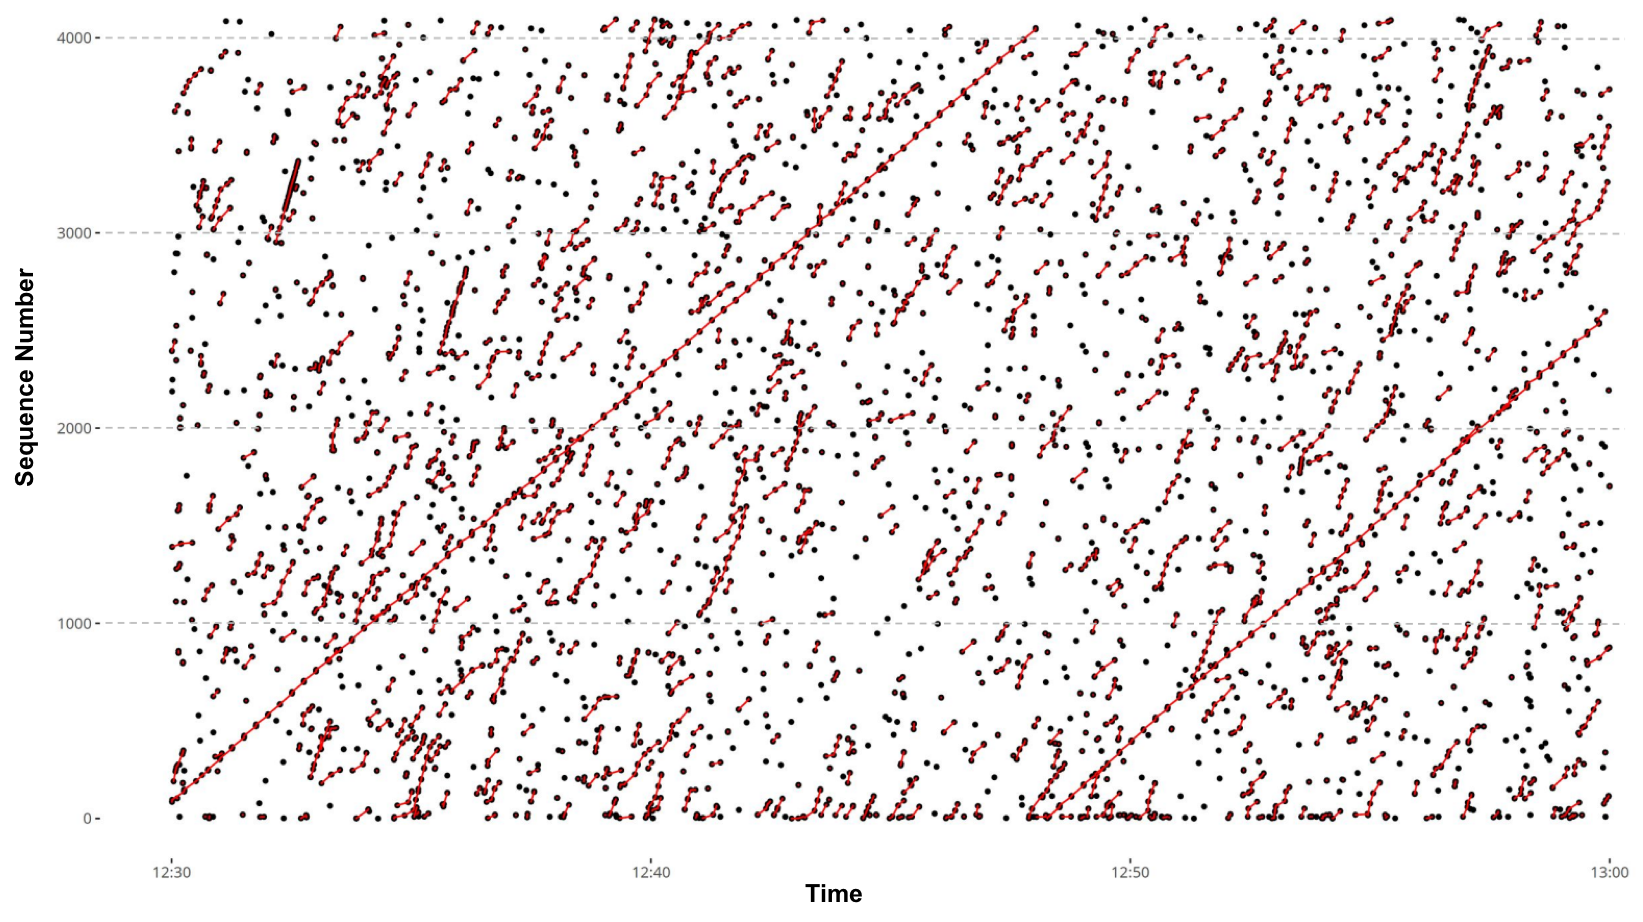
\includegraphics [width=0.85\linewidth,trim=4 4 4 4,clip] {images/methodology_clustering.png}
		\caption{Clustering probe requests based on increasing sequence numbers present in them.}
		\label{clustering_pilot}
	\end{center}
\end{figure}

Figure \ref{clustering_pilot} shows the clustering process: 
the black dots show the probe requests and the red lines 
connect them into clusters representing those which were
generated by the same device.
We finally combined both normal and anonymised probe requests,
aggregated them based on their unique identifier, and
removed repeating probe requests which reduced the difference
between the sensor counts and the manual counts to -18\%.

\begin{figure}
	\begin{center}
		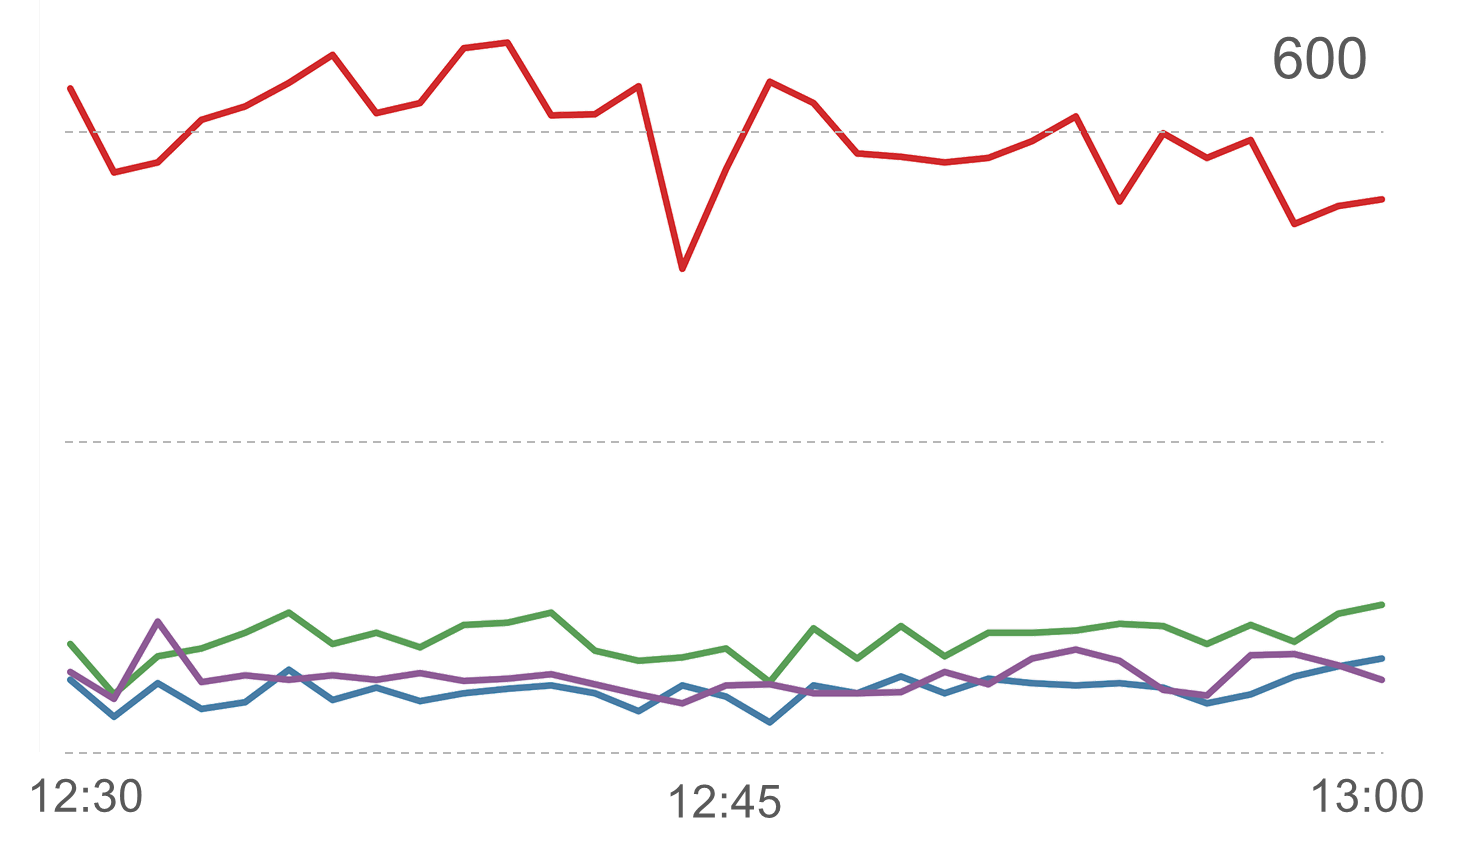
\includegraphics [width=0.85\linewidth] {images/pilot_counts_comparision.png}
		\caption{Comparision of counts after filtering with manual counts}
		\label{comparision_pilot}
	\end{center}
\end{figure}

we find that the methodology works as shown by the reduction in the
mean error
We find kmeans and quantile best algorithms for filtering
sequencing works. Even in densely populated areas.

Though this is promising we need to know more to generalise the methodology.
we do a detailed multi location, longer term study with multiple manual
verification which is the main study.

	\section{Main Study}\label{main_study}
		The aims of the main study are,
test the validity of the signal strength algorithm in different 
micro site conditions.
Test that the sequence number algorithm works in real world
for different locations and different times.
check if the thresholds are consistent.
Test if the calibration works over intervals
Finally conclude if we can estimate footfall confidently
with just probe requests.

five locations were selected across central london which
had different types of configurations and specific problems
configuratons are shown in fig. map is shown in figure.
\begin{enumerate}
	\item Phone Shop Camden - has phones and bus stops.
	\item Restaurant TCR - has seating area on either side.
	\item Holborn Information Kiosk - High volumne station entry
	\item Restaurant Russell Square - seating on one side and side walk on other
	\item Shop Charring Cross - sidewalk on one side and phone shop next door
\end{enumerate}
Installations were carried out over the time period from xxxx to xxxx.
the data collection happened from xxxx to xxxx. Manual counting was carried out
with high precision on dates xxxx and aggregated five minutes on xxxx.
The difference in methods could lead to some inaccuracies in data.
The overall schedule is shown in half page graphic.

The overall statistics of data collected. How many probe requests.
Comparision of location in terms of volume, patterns in daily footfall etc.
The comparision between global and local.
comparision between different types of vendors.
Specifics on top 5 manufacturers.

We do a daily analysis of distribution of signal strengths.
The thresholds are shown in the table.
The average is xxxx and standard deviation is xxx.
we notice that the variation is lot. There is a definite
change with the micro site locations.

We see how the signal strength filtering affects the counts.
compared to manual counts we look at the average mean errors (daily)
per 5 minutes. The counts go as follows.
Shown as a red line in the Figure.

We can conclude that even though it has variations, this is
a good method to reduce the overall level of error.

This is also done for different locations hourly for all the data we had.
we compare it to the manual counts and see that the average mean error
has been reduced/increased. The finger print works well for all the locations.
It also works over a period of time and gives us a comparable and close 
footfall count to the manual count. The thresholds found in the pilot study
works as well.

Finally we normalise the sensor counts to match the manual count using
a fraction/ adjustment factor calculated from the know manual counts.
we have three sets of counts. We check if the adjustment factor holds the
same in all three counts across locations. It does with a variations from
xxx to xxx. The results are shown in the table. 

we see that the signal strength filtering works and reduces error by
xxxxx. there is variation by locations.
we see that sequence number algorithm works as well. The threshold stays
constant well and works well across locations. The calibration also works
and ajustment factor stays consistent short term. This needs more work 
long term.

	\section{Conclusion}\label{conclusion}
		Sentient technologies make measurement of the human activities that are the life
blood of the smart city possible. Yet the data that they harvest are frequently
relevant only to the sub-groups within society that avail themselves of
particular goods and services – such as social media applications, transport
modes or retail offers. In each of these cases, it is necessary to remember that
the resulting data are by-products of consumer transactions, and will as a
consequence, only pertain to users of the relevant goods or services. If the
smart city is to be socially inclusive, it therefore follows that sentient data
must represent entire populations, whether by design or by triangulation with
external, population wide, sources. This is a non-trivial task, since the ebbs
and flows of smart device-enabled citizens rarely pertain to any clearly defined
population in either administrative or functional terms
\citep{massam1975location}.

Our objective here has been to collect, rather than re-use, data on smart city
functioning, by recording Wi-Fi probes and ultimately reconciling them with
manual counts in order to infer ambient populations. The internal validation
methodology set out in the technical sections of this paper, allied to external
validation from pedestrian counts, renders the method inclusive and robust when
recording activity levels in retail centres in real time. We have described the
collection and processing of a novel consumer Big Dataset that enables valid
measures of levels of footfall activity which has been scaled across a wide
network of sensors \citep{cdrc2018consumer}.  In both conceptual and technical
terms, it illustrates the ways in which passively collected consumer data can be
‘hardened’ to render them robust and reliable by using related procedures of
internal and external validation.

Internal validation addresses the issues of screening out device probes that do
not indicate footfall, and the further screening of device probes to
‘fingerprint’ the effects of MAC randomization. It is important to note that the
filtering process work based solely on the information present in the probe
requests and their temporal distribution. This ensures that although the mobile
devices were uniquely identified, there was no further personal data generated
by linking the probe requests to the users of the mobile devices. This method
essentially gave us a way to estimate the footfall in real-time without
identifying or tracking the mobile devices themselves. External validation then
entailed reconciling adjusted counts with the footfall observed at sample
locations. This procedure makes it possible to generalise from locations at
which manual footfall surveys are conducted to all others in the system, and to
develop a classification of device locations that are more or less susceptible
to noise generation.

This Wi-Fi based footfall counting methodology offers a large number of
applications and benefits for real time spatial analysis. Since Wi-Fi based
sensors are inexpensive and the data model is scalable, it is possible to use
this methodology for a large network of sensors to gather granular data on
pedestrian footfall. A snapshot showing a week’s worth of precise footfall in
area around Charring cross, London is shown in Figure \ref{main_study_counts} in
order to demonstrate the potential for such a dataset. Projects such as
SmartStreetSensors \citep{cdrc2018consumer}, may utilise this methodology to
overcome the challenges introduced by the implementation of MAC address
randomisation.

The vicissitudes of MAC randomisation, and the provisions of privacy
legislation such as EU General Data Protection Regulations mitigate against
tracking individuals across the smart city using this approach.  This can be
modelled using agent-based methods \citep{heppenstall2011agent}, however. In
our own research we have also begun to link store time-lagged till receipts to
footfall, and have used such data to better understand the dwell times that
characterise such different retail uses as stores with window displays and fast
food restaurants.  Such analysis not only provides a more nuanced picture of
movement through retail areas, but also enables valorisation of micro sites
within retail centres. In the UK, for example, this is of immediate practical
importance in evaluating business rates on properties, and has still wider
implications for the setting of retail unit rental values. There are obvious
extensions to understanding the ebbs and flows of activities in the 24-hour
smart city such as understanding urban mobility \citep{gariazzo2019spatio} and
conceptualising them with a people dimension \citep{nam2011conceptualizing}.

More broadly still, extensions to this strand of smart city research are likely
to seek to differentiate the quality of different elements within footfall
according to mission e.g. travel to adjacent workplace zones, leisure, etc., and
personal characteristics such as spending power. In this respect, future
research may not only simulate linkage of harmonised footfall counts between
sensor locations, but also link these in turn to disaggregate origin-destination
matrices for bikeshare and other public transport modes.  Our own investigations
will consider these and other challenges to understanding the functioning of the
sentient city.

	\section*{Acknowledgement}
		This research was funded by Economic Social Research Council grant – Retail
Business Datasafe (ES/L011840/1) through Consumer Data Research Centre.  Authors
would like to acknowledge the contributions of the Local Data Company in
facilitating the data collection process and Dr Roberto Murcio and Dr Tank Green
for their inputs.

	\bibliographystyle{tfv} \bibliography{references}

\end{document}
